\subsection{Continuous phase of walker}

\subsubsection*{Forward Kinematics}
\begin{align}
	x_1 &= \frac{l_1}{2}\cos\theta_1\nonumber \\
	\dot{x_1} &= -\frac{l_1}{2}\sin(\theta_1)\dot{\theta}_1\nonumber \\
	y_1 &= \frac{l_1}{2}\sin\theta_1\nonumber \\
	\dot{y_1} &= \frac{l_1}{2}\cos(\theta_1)\dot{\theta}_1\nonumber \\
	x_2 &= l_1\cos\theta_1 + \frac{l_2}{2}\cos(\theta_1 + \theta_2)\nonumber \\
	\dot{x_2} &= -l_1\sin(\theta_1)\dot{\theta}_1 - \frac{l_2}{2}\sin(\theta_1 + \theta_2)(\dot{\theta}_1 + \dot{\theta}_2)\label{eqn:x2dot} \\
	y_2 &= l_1\sin\theta_1 + \frac{l_2}{2}\sin(\theta_1 + \theta_2)\nonumber \\
	\dot{y_2} &= l_1\cos\theta_1\dot{\theta}_1 + \frac{l_2}{2}\cos(\theta_1 + \theta_2)(\dot{\theta}_1 + \dot{\theta}_2)\label{eqn:y2dot}
\end{align}  
\subsubsection*{Lagrangian Dynamics}
In order to produce the dynamical equations for the two-link manipulator, we must compute the Lagrangian:
\begin{align}
	L &= K - P\nonumber \\
	T_i &= \frac{\partial}{\partial{t}}\left(\frac{\partial{L}}{\partial{\dot{\theta}_i}}\right) - \frac{\partial{L}}{\partial{\theta_i}}\label{eqn:T_i}
\end{align}
The kinetic energy of the manipulator is given by the summation of the pure rotational kinetic energy of the first link about the origin and the rotational kinetic energy of the second link about its centre and the linear KE of its centre of mass.
\begin{align}
	K &= \frac{1}{2}I_1\dot{\theta}_1^2 + \frac{1}{2}I_2(\dot{\theta}_1 + \dot{\theta}_2)^2 + \frac{1}{2}m_2 V_2^2\label{eqn:KE}
\end{align}
From equations \ref{eqn:x2dot} and \ref{eqn:y2dot}, we have expressions for the components of $V_2$:
\begin{align*}
	V_2^2 &= \left[l_1^2 s_1^2 \dot{\theta}_1^2 + l_1 l_2 s_1 s_{12} \dot{\theta}_1(\dot{\theta}_1 + \dot{\theta}_2) + \frac{l_2^2}{4} s_{12}^2(\dot{\theta}_1 + \dot{\theta}_2)^2\right] \\
	& + \left[l_1^2 c_1^2 \dot{\theta}_1^2 + l_1 l_2 c_1 c_{12} \dot{\theta}_1(\dot{\theta}_1 + \dot{\theta}_2) + \frac{l_2^2}{4} c_{12}^2(\dot{\theta}_1 + \dot{\theta}_2)^2\right]
\end{align*}
Combining terms and exploiting the trigonometric identities $\sin^2{x} + \cos^2{x} = 1$ and $\cos(x - y) = \cos{x}\cos{y} + \sin{x}\sin{y}$:
\begin{align}
	V_2^2 &= l_1^2 \dot{\theta}_1^2 + l_1 l_2 c_2 \dot{\theta}_1(\dot{\theta}_1 + \dot{\theta}_2) + \frac{1}{4}l_2^2(\dot{\theta}_1 + \dot{\theta}_2)^2\label{eqn:V_2}
\end{align}
Substituting equation \ref{eqn:V_2} into equation \ref{eqn:KE}:
\begin{align}
	K =& \frac{1}{2}I_1\dot{\theta}_1^2 + \frac{1}{2}I_2\left(\dot{\theta}_1 + \dot{\theta}_2\right)^2\nonumber \\
	& + \frac{1}{2}m_2\left[\dot{\theta}_1^2\left(l_1^2 + \frac{1}{4}l_2^2 + l_1 l_2 c_2\right) + \dot{\theta}_2^2\left(\frac{1}{4}l_2^2\right) + \dot{\theta}_1\dot{\theta}_2\left(\frac{1}{2}l_2^2 + l_1 l_2 c_2\right)\right]\nonumber \\
	P =& \frac{1}{2}l_1 s_1 m_1 g + \left(l_1 s_1 + \frac{1}{2}l_2 s_{12}\right)m_2 g\nonumber \\
	L =& \frac{1}{2}\dot{\theta}_1^2 \left(I_1 + I_2 + m_2\left(l_1^2 + \frac{1}{4}l_2 + l_1 l_2 c_2 \right) \right) + \frac{1}{2}\dot{\theta}_2^2\left(I_2 + \frac{1}{4}m_2 l_2^2 \right)\nonumber \\
	& + \dot{\theta}_1\dot{\theta}_2 \left(I_2 + \frac{1}{2}m_2 \left(\frac{1}{2}l_2^2 + l_1 l_2 c_2 \right) \right) - \frac{1}{2}l_1 s_1 m_1 g - \left(l_1 s_1 + \frac{1}{2}l_2 s_{12}\right)m_2 g\label{eqn:L}
\end{align}
Now, we can determine equations for the torques using equations \ref{eqn:T_i} and \ref{eqn:L}.
\begin{align*}
	\frac{\partial{L}}{\partial{\dot{\theta}_1}} =& \dot{\theta}_1\left(I_1 + I_2 + m_2 \left(l_1^2 + \frac{1}{4}l_2^2 + l_1 l_2 c_2 \right) \right) + \dot{\theta}_2 \left(I_2 + \frac{1}{2}m_2 \left(\frac{1}{2}l_2^2 + l_1 l_2 c_2 \right) \right) \\
	\frac{\partial}{\partial{t}}\left(\frac{\partial{L}}{\partial{\dot{\theta}_1}}\right) =& \ddot{\theta}_1 \left(I_1 + I_2 + m_2\left(l_1^2 + \frac{1}{4}l_2^2 + l_1 l_2 c_2 \right) \right) - \dot{\theta}_1 \dot{\theta}_2 \left(m_2 l_1 l_2 s_2 \right) \\
	&+ \ddot{\theta}_2 \left(I_2 + \frac{1}{2}m_2\left(\frac{1}{2}l_2^2 + l_1 l_2 c_2 \right)\right) - \dot{\theta}_2^2 \left( \frac{1}{2} m_2 l_1 l_2 s_2 \right) \\
	\frac{\partial{L}}{\partial{\theta_1}} =& -\frac{1}{2}l_1 c_1 m_1 g - m_2 g \left(l_1 c_1 + \frac{1}{2}l_2 c_{12} \right)
\end{align*}
Adding the components together, we get:
\begin{align}
	T_1 =& \ddot{\theta}_1 \left(I_1 + I_2 + m_2\left(l_1^2 + \frac{1}{4}l_2^2 + l_1 l_2 c_2 \right) \right) - \dot{\theta}_1 \dot{\theta}_2 \left(m_2 l_1 l_2 s_2 \right)\nonumber \\
	&+ \ddot{\theta}_2 \left(I_2 + \frac{1}{2}m_2\left(\frac{1}{2}l_2^2 + l_1 l_2 c_2 \right)\right) - \dot{\theta}_2^2 \left( \frac{1}{2} m_2 l_1 l_2 s_2 \right)\nonumber \\
	&+ \frac{1}{2}l_1 c_1 m_1 g + m_2 g \left(l_1 c_1 + \frac{1}{2}l_2 c_{12} \right)\label{eqn:T1}
\end{align}
Likewise for $T_2$:
\begin{align*}
	\frac{\partial{L}}{\partial{\dot{\theta}_2}} =& \dot{\theta}_2 \left(I_2 + \frac{1}{4}m_2 l_2^2 \right) + \dot{\theta}_1 \left(I_2 + \frac{1}{2}m_2 \left(\frac{1}{2}l_2^2 + l_1 l_2 c_2 \right) \right) \\
	\frac{\partial}{\partial{t}}\left(\frac{\partial{L}}{\partial{\dot{\theta}_2}}\right) =& \ddot{\theta}_2\left(I_2 + \frac{1}{4}m_2 l_2^2 \right) + \ddot{\theta}_1\left(I_2 + \frac{1}{2}m_2 \left(\frac{1}{2}l_2^2 + l_1 l_2 c_2 \right) \right) - \dot{\theta}_1 \dot{\theta}_2 \left(\frac{1}{2}m_2 l_1 l_2 s_2 \right) \\
	\frac{\partial{L}}{\partial{\theta_2}} =& - \dot{\theta}_1^2 \left(\frac{1}{2}m_2 l_1 l_2 s_2 \right) - \dot{\theta}_1\dot{\theta}_2 \left(\frac{1}{2} m_2 l_1 l_2 s_2 \right) - \frac{1}{2} m_2 g l_2 c_{12}
\end{align*}
Adding components as for $T_1$:
\begin{align}
	T_2 =& \ddot{\theta}_2\left(I_2 + \frac{1}{4}m_2 l_2^2 \right) + \ddot{\theta}_1\left(I_2 + \frac{1}{2}m_2 \left(\frac{1}{2}l_2^2 + l_1 l_2 c_2 \right) \right)\nonumber \\
	&+ \dot{\theta}_1^2 \left(\frac{1}{2}m_2 l_1 l_2 s_2 \right) + \frac{1}{2} m_2 g l_2 c_{12}\label{eqn:T2}
\end{align}

Thus we have an equation of the form
\begin{equation}
	M\left(q(t)\right)\ddot{q}(t) + C\left(q(t),\dot{q}(t)\right)\dot{q}(t)
	 + G\left(q(t)\right) = B\left(q(t)\right)u(t)
\end{equation} where
\begin{eqnarray*}
	M\left(q(t)\right) &=& \begin{bmatrix}
		I_1 + I_2 + m_2\left(l_1^2 + \frac{1}{4}l_2^2 + l_1l_2\cos{q_2}\right) &
		I_2 + \frac{1}{2}m_2\left(\frac{1}{2}l_2^2 + l_1l_2\cos{q_2}\right) \\
		I_2 + \frac{1}{2}m_2\left(\frac{1}{2}l_2^2 + l_1l_2\cos{q_2}\right) &
		I_2 + \frac{1}{4}m_2l_2^2
	\end{bmatrix} \\
	C\left(q(t),\dot{q}(t)\right) &=& \begin{bmatrix}
		-m_2 l_1 l_2 \sin({q_2}) \dot{q}_2 &
		-\frac{1}{2}m_2 l_1 l_2 \sin({q_2}) \dot{q}_2 \\
		\frac{1}{2}m_2 l_1 l_2 \sin({q_2}) \dot{q}_1 & 0
	\end{bmatrix} \\
	G\left(q(t)\right) &=& \begin{bmatrix}
		\frac{1}{2}l_1 \cos{q_1} m_1 g + m_2 g \left(l_1 \cos{q_1} + \frac{1}{2}l_2 \cos{(q_1 + q_2)} \right) \\
		\frac{1}{2} m_2 g l_2 \cos{(q_1 + q_2)}
	\end{bmatrix} \\
	B\left(q(t)\right) &=& \begin{bmatrix}
		0 \\ 1
	\end{bmatrix}, ~
	u(t) = T_2, ~
	q(t) = \begin{bmatrix}
		q_1(t) \\ q_2(t)
	\end{bmatrix}
\end{eqnarray*}

\subsection{Impact dynamics}
Following the derivation as presented by Westervelt \cite{westervelt2007feedback}, the full-state impact dynamics are of the form: \\
\begin{eqnarray}
	q\left(t^+\right) &=& Rq\left(t^-\right) \\
	\dot{q}\left(t^+\right) &=& R\Delta\left(q\left(t^-\right)\right)\dot{q}\left(t^-\right)
\end{eqnarray}

The condition for impact for walking on flat ground is $\theta_2 = -2 \theta_1$ AND $\theta_2 < -180 + \epsilon$, where $\epsilon$ is chosen such that the shortest footstep is possible. The second condition assumes that it is not possible to step backwards. This is reasonable, since the current objective is to construct feasible forward-walking motion. \\ \par

\begin{figure}[htp]
	\centering
	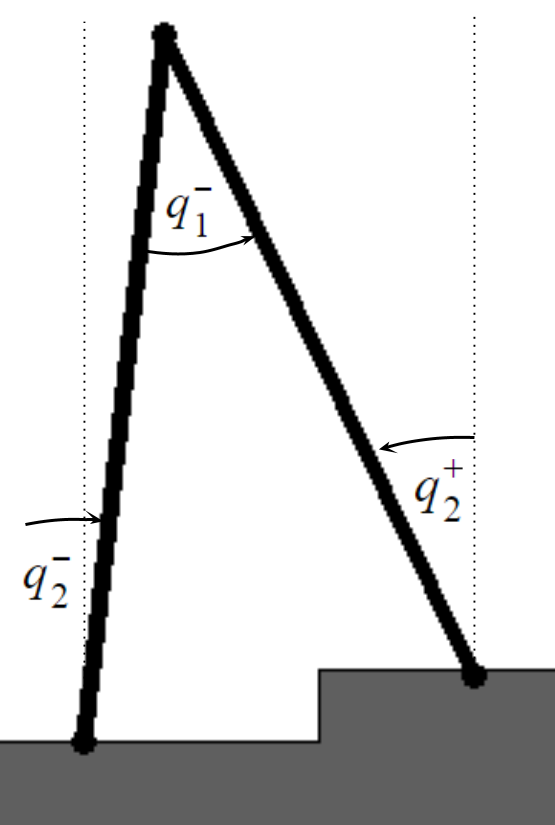
\includegraphics[scale=1]{../images/impact.png}
	\caption{Change of coordinates at impact}
	\label{fig:changecoords}
\end{figure}

The change of coordinates at impact is depicted in Figure~\ref{fig:changecoords}. It can be trivially shown that $\theta_1^* = \pi - \theta_1$ and that $\theta_2^* = 2\pi - \theta_2$. In order to find the derivatives of $\theta_1^*$ and $\theta_2^*$, we examine the general form of these angles (i.e. at non-specific angle values). It is not difficult to derive that $\theta_1^* = \theta_1 + \theta_2 + \pi$ and it is noted that $\theta_2^* = 2\pi - \theta_2$ in general. Thus $\dot{\theta}_1^* = \dot{\theta_1} + \dot{\theta}_2$ and $\dot{\theta}_2^* = -\dot{\theta}_2$. \\

If we assume that angular momentum is conserved, i.e. $L^+ = L^-$, where
\begin{eqnarray*}
	L^- &=& I_1\dot{\theta}_1 + I_2\left(\dot{\theta}_1 + \dot{\theta}_2\right) \\
	L^+ &=& I_1\dot{\theta}_1^* + I_2\left(\dot{\theta}_1^* + \dot{\theta}_2^*\right)
\end{eqnarray*}
\par Substituting values for $\dot{\theta}_1^*$ and $\dot{\theta}_2^*$, we get
\begin{equation}
	\dot{\theta}_1^+\left(I_1 + I_2\right) + \dot{\theta}_2^+\left(I_1\right)
	= \dot{\theta}_1^-\left(I_1 + I_2\right) + \dot{\theta}_2^-\left(I_2\right)
\end{equation}
This equation does not yet yield a solution for $\theta_1^+, \theta_2^+$, since we at this stage need one to find the other.